\documentclass[a4paper, 12pt]{article}
\usepackage[protrusion=true,expansion=true]{microtype} % Better typography
\usepackage[top=0.5in, bottom=0.75in, left=0.625in, right=0.625in]{geometry}

\usepackage{graphicx} % Required for including pictures
\usepackage{float}
\usepackage{wrapfig} % Allows in-line images

% \usepackage{mathpazo} % Use the Palatino font
\usepackage[T2A]{fontenc}
\usepackage[utf8]{inputenc}
\usepackage[english,russian]{babel}
\usepackage[style=gost-numeric]{biblatex}
\usepackage{indentfirst}
\usepackage[colorlinks=true, urlcolor=blue, citecolor=black]{hyperref}

%%% Дополнительная работа с математикой
\usepackage{amsmath,amsfonts,amssymb,amsthm,mathtools} % AMS
\usepackage{icomma} % "Умная" запятая: $0,2$ --- число, $0, 2$ --- перечисление

%% Номера формул
\mathtoolsset{showonlyrefs=true} % Показывать номера только у тех формул, на которые есть \eqref{} в тексте.

%% Шрифты
\usepackage{euscript}	 % Шрифт Евклид
\usepackage{mathrsfs} % Красивый матшрифт

%% Свои команды
\DeclareMathOperator{\sgn}{\mathop{sgn}}

%% Перенос знаков в формулах (по Львовскому)
\newcommand*{\hm}[1]{#1\nobreak\discretionary{}
	{\hbox{$\mathsurround=0pt #1$}}{}}

\usepackage{graphicx}
\graphicspath{ {images/} }

\linespread{1.5} % Change line spacing here, Palatino benefits from a slight increase by default


\begin{document}


\begin{titlepage}

\newcommand{\HRule}{\rule{\linewidth}{0.5mm}} % Defines a new command for the horizontal lines, change thickness here

\center % Center everything on the page

%----------------------------------------------------------------------------------------
%	HEADING SECTIONS
%----------------------------------------------------------------------------------------
{\Large Федеральное государственное автономное образовательное учреждение
	высшего образования}\\[1.0cm]
{\LARGE <<Национальный исследовательский университет 
	<<Высшая школа экономики>>}\\[0.5cm] % Name of your university/college

{\Large Факультет компьютерных наук\\
	ОП «Прикладная математика и информатика»}\\[1.5cm] % Minor heading such as course title


%----------------------------------------------------------------------------------------
%	TITLE SECTION
%----------------------------------------------------------------------------------------


{ \huge \bfseries Отчет о прохождении практики}\\ % Title of your document


%----------------------------------------------------------------------------------------
%	AUTHOR SECTION
%----------------------------------------------------------------------------------------

% If you don't want a supervisor, uncomment the two lines below and remove the section above
\begin{flushleft}
  \large \textbf{Студент:} \
   Гайдамашко Даниил Олегович\\% Your name
   \large \textbf{Группа:} \
   БПМИ-165\\% Your name
   \large \textbf{Вид практики:} \
   учебная\\
    \textbf{Организация:} \
   НИУ ВШЭ\\% Your name
\end{flushleft}

%----------------------------------------------------------------------------------------
%	DATE SECTION
%----------------------------------------------------------------------------------------
\vfill\vfill\vfill\vfill\vfill

\large \textbf{Руководитель практики:} Конушин Антон Сергеевич \hrulefill\\[2cm]

{\large \today}\\[2cm] % Date, change the \today to a set date if you want to be precise


\vfill % Fill the rest of the page with whitespace

\end{titlepage}

{
\hypersetup{linkcolor=black}
\tableofcontents
}

\newpage

\section*{Вступление.}
\addcontentsline{toc}{section}{\protect\numberline{}Вступление.}%

Колоссальную роль в жизни человека играет психологический процесс восприятия окружающего мира --  целостного отражения предметов и явлений объективного мира при их непосредственном воздействии на органы чувств. И большинство людей составляют значительную часть картины окружающей действительности при помощи зрения -- способности воспринимать имформацию путём преобразования энергии электромагнитного излучения светового диапазона, осуществляемая зрительной системой.

Помимо формирования изображения, отражающего состояние окружающего нас мира в данный момент времени, задача зрения состоит и в его анализе, а именно, выделении объектов, определении их признаков и атрибутов.

Компьютерное зрение -- это одна из областей искусственного интеллекта (AI), задача которой -- построение компьютерной модели зрительной системы, выполняющей данные функции, и использование полученной информации об изображениях в прикладных целях. В настоящее время эта область знаний вляется молодой, разнообразной и быстроразвивающейся.

В рамках данной практики было предложено познакомиться с основами компьютерного зрения и машинного обучения -- одного из метода решения задач данной области знаний.

Целями учебной практики являются:
\begin{enumerate}
\item Изучение основных понятий и теоретической базы области компьютерного зрения, рассмотрение способов обработки изображений, а также ознакомление с основами машинного обучения;
\item Повышение навыков программирования на языке Python, получение опыта работы со специализированными библиотеками языка Python для научных вычислений и задач анализа данных;
\end{enumerate}

Задачами учебной практики являются:
\begin{enumerate}
\item Изучение учебных материалов по компьютерному зрению -- 5 видеолекций курса А.С. Конушина <<Введение в компьютерное зрение и глубинное обучение>>;
\item Выполнение 3 практических заданий по обработке и распознаванию изображений на языке программирования Python;
\end{enumerate}

\newpage
\section*{Основная часть}
\addcontentsline{toc}{section}{\protect\numberline{}Основная часть.}%

Прохождение учебной практики осуществлялось дистанционно с <<1>> июля по <<31>> августа 2017 г. Руководитель практики предоставил возможность свободного графика, поэтому непосредственное выполнение практических заданий у меня пришлось на август. Инструментом прохождения практики был портал \textbf{cv-gml.ru}, который содержал как ссылки на учебные материалы, так и тестирующую систему, автоматически проверяющую загруженные решения.

В ходе учебной практики была проделана работа над практическими заданиями:
\begin{enumerate}
\item \textbf{Совмещение каналов изображения (<<Проскудин-Горский>>)} \\-- реконструкция изображений Прокудина-Горского;
\item \textbf{Контекстно-зависимое масштабирование изображений (<<Умный ресайз>>)} \\-- изменение пропорций изображений с сохранением содержания;
\item \textbf{Распознавание автодорожных знаков} \\-- распознавание дорожных знаков с помощью метода SVM;
\end{enumerate}

\subsection*{Практическое задание <<Совмещение каналов изображения>>}
\addcontentsline{toc}{subsection}{\protect\numberline{}Практическое задание <<Совмещение каналов изображения>>}%

Данное задание напрямую связано с понятием цифрового цветного изображения, с которым было предложено ознакомиться в ходе первой лекции. Цифровое цветное изображение -- это
трёхмерная матрица (тензор ранга 3), в котором для каждого пиксела (x,y) хранится цвет, который описывается вектором <<каналов>>. Обычно каждая компонента дискретизируется до [0,255] в 8 бит. Существуют разные варианты моделей, при помощи которых описывается цвет. Среди них выделяются линейные модели, основанные на выборе базовых цветов и их
линейных комбинациях. Одной из них является модель RGB с красным, зеленым и синим базовыми цветами.

Задание посвящено российскому изобретателю С.М. Проскудину-Горскому -- пионеру цветной фотографии в России. Он использовал технологию цветоделения, придуманную Дж. Максвеллом в середине XIX века, которая заключалась в разделении света сложного спектрального состава на несколько монохромных полутоновых составляющих. Съёмка велась по очереди через цветные светофильтры синего, зелёного и красного цветов, после чего получались три чёрно-белых негатива, пригодные для аддитивной проекции на экран.

Задание заключается в реализации процесса соединения трех полутоновых RGB-составляющих в цветную картину. На вход алгоритма поступает дефектная полутоновая фотография вертикально расположенных фотокарточек каждого канала, а также координаты некоторой точки с зеленого негатива. На выходе алгоритм выдает координаты точек красного и синего негативов, которые наложились на заданную при оптимальном совмещении каналов (при оптимальном сдвиге слоев друг относительно друга).

Мною был реализован следующий алгоритм, решающий данную задачу:
\begin{enumerate}
	\item Загрузка изображения и разделение изображения на три канала (разделение изоб
	ражения на три равные части по высоте);
	\item Удаление рамок пленки (обрезание полученных изображений  на 5\% с каждой стороны);
	\item Поиск наилучшего сдвига для совмещения каналов (поиск наилучшего совмещения красной и зеленого каналов, а затем зеленого и синего);
\end{enumerate}

Для того, чтобы совместить два канала изображения, производился сдвиг красного или синего относительно зеленого в пределах от -15 до 15 пикселей. Для перекрывающихся областей изображений подсчитывалась метрика, и наилучшим совмещением являлся сдвиг с оптимильнейшим значением метрики. Предлагалось реализовать две метрики и выбрать ту,
которая позволяет получить более качественный результат при совмещении:
\begin{enumerate}
\item Среднеквадратичное отклонение для изображений $I_1$ и $I_2$ :
\[MSE(I_1 , I_2) =\frac{1}{width\cdot height}\cdot
\sum_{x, y}^{} (I_1 (x, y) - I_2 (x, y))^2
\]
где $width$, $height$ -- ширина и высота изображений соответственно. Для нахождения опти-
мального сдвига нужно взять минимум по всем сдвигам.

\item Нормализованная кросс-корреляция для изображений $I_1$ и $I_2$ :
\[I_1*I_2 =\frac
{\sum_{x, y}^{} I_1(x, y) \cdot I_2(x, y)}
{\sqrt{\sum_{x, y}^{} I_1^2(x, y)\cdot 
		\sum_{x, y}^{} I_2^2(x, y)}}
\]
Для нахождения оптимального сдвига нужно взять максимум по всем сдвигам.
\end{enumerate}

Было замечено, что использование нормализованной кросс-корреляции дает чуть меньшие отклонения от оптимальных решений из тестовых данных.

Опциональным заданием являлась реализация совмещение при помощи пирамиды изображений для ускорения работы алгоритма на больших изображениях. В пирамиде изображений исходное изображение последовательно уменьшается в 2 раза до некоторого размера (чтобы
обе стороны были не больше 500 пикселей в длину). Поиск оптимального сдвига начинается с самого
маленького изображения, а затем на пути к исходному изображению уточняется на уменьшенных
копиях изображения. То есть, если для уменьшенной в 2 раза копии изображения был найдем сдвиг $\varepsilon$, до для самого изображения сдвиг уточняется в диапозоне $[-2+\varepsilon/2, \varepsilon/2+2]$.

Таким образом, оригинальное изображение совмещается не в диапазоне
[-15, 15] пикселей, а в меньшем, уточненном с помощью уменьшенных копий изображения.

Для реализации данной подзадачи была написана рекурсивная функция, зависящая от размера изображений и, которая запускала стандартный алгоритм поиска оптимального сдвига в диапозоне [-15, 15] пикселей для изображений, обе стороны которых не больше 500 пикселей в длину, либо запускалась рекурсивно для умньшенных вдвое копий изображений, и для каждого найденного сдвига $\varepsilon_i$ запускала стандартный алгоритм поиска сдвига в диапозоне [$-2+\varepsilon_i/2$, $\varepsilon_i/2+2$] для текущего масштаба.

В результате выполнения данного задания я научился эффективно работать с объектами линейной алгебры при помощи библиотеки \textbf{NumPy}, которая, благодаря встроенным функциям, написанным на языке C, помогает ускорить процесс вычислений, нежели это была бы обычная реализация с циклами на Python.

\newpage

\subsection*{Практическое задание\\ <<Контекстно-зависимое масштабирование изображений>>}
\addcontentsline{toc}{subsection}{\protect\numberline{}Практическое задание <<Контекстно-зависимое масштабирование изображений>>}%

В данном задании предлагается реализовать алгоритм, применяющийся для контекстно-зависимого
масштабирования изображений. При стандартном подходе изображение равномерно деформируется
по всей длине при изменении размера (объекты на изображении уменьшаются вместе со всем
изображением). Данный же алгоритм учитывает контекст, и деформация происходит так, что
объекты сохраняют свои размеры. Кроме того, если с помощью маски выделить какой-нибудь объект,
то его можно удалить из изображения или наоборот оставить неизменным.

\begin{figure}[h]
	\centering
	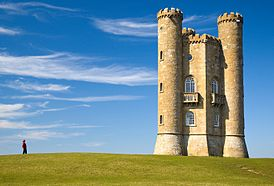
\includegraphics[scale=2]{sc1.jpg}
	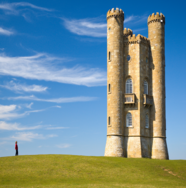
\includegraphics[scale=0.6]{sc2.png}
	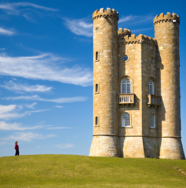
\includegraphics[scale=0.6]{sc3.png}
	\caption{Оригинальное изображение, обычное сжатие, умное сжатие}
\end{figure}

Алгоритм решения данной задачи состоит в работе со швами -- связанными кривыми, верхнюю и нижнюю или правую или левую границы изображения. А сами швы предлагается искать в матрице энергий каждого пикселя изображения. Хотя под понятием энергии каждой точки могут подразумеваться разные вещи, в задании было предложено аппеллировать к понятию модуля градиента яркости в данной точке. Идея состоит в том, что 
если шов проходит через малое количество перепадов яркости, это означает, что он имеет малую
энергию. А так как объекты обычно имеют более сложную структуру, чем фон, то швы,
которые будут проходить через них, будут иметь более высокую энергию, следовательно мы их не
удалим.

\begin{figure}[h]
	\centering
	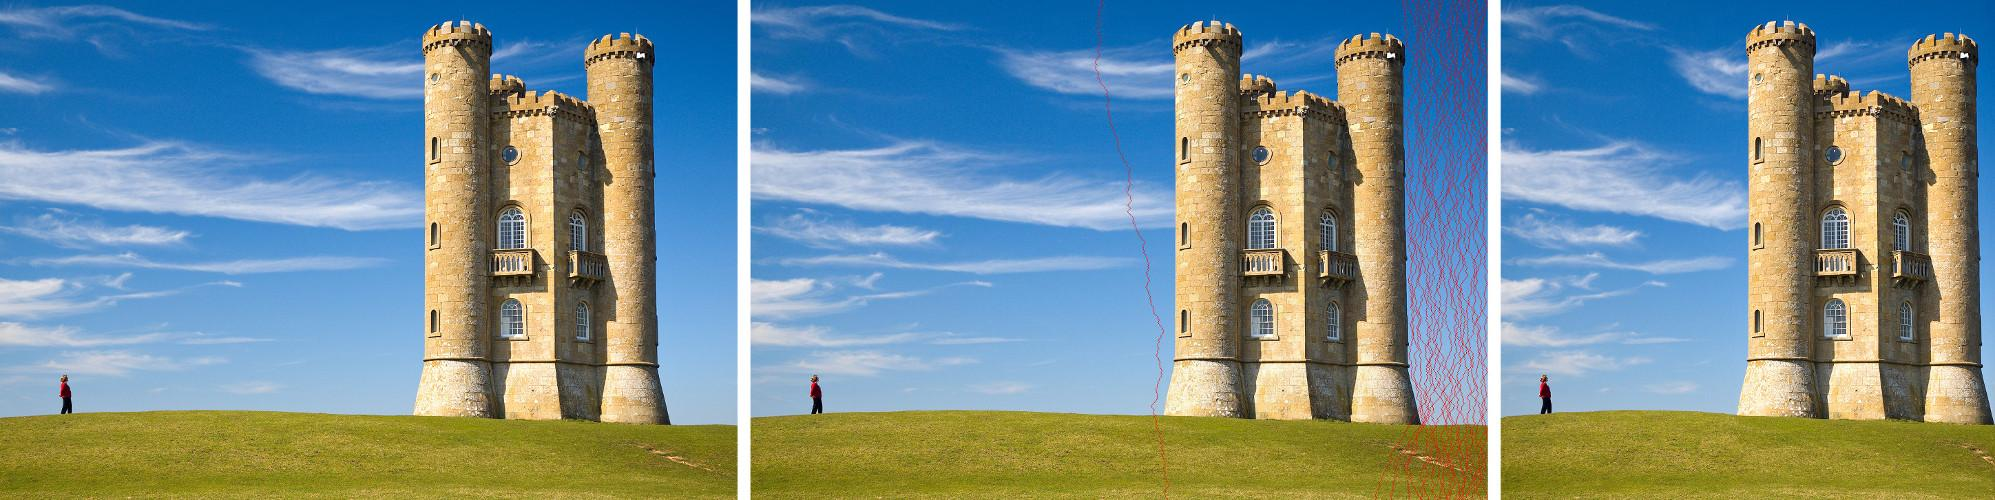
\includegraphics[scale=0.2]{resize_diff.jpeg}
	\caption{Алгоритм находит швы в наименее детализированных частях изображения}
\end{figure}

Таким образом, алгоритм контекстно-зависимого масштабирования заключается в нахождении шва с наименьшей энергией, то есть наименее детализированной части изображения. Был реализован следующий алгоритм нахождения такого шва:
\begin{enumerate}
	\item Конверсия 3-канального RGB-изображения в компаненту яркости цветовой модели YUV по формуле:\[Y=0.299\cdot R + 0.587\cdot G + 0.114\cdot B\]
	\item Вычисление нормы градиента в каждой точке (корень из суммы квадратов
	частных производных по каждому из направлений)
	\item Нахождения минимального шва при помощи динамического программирования.
\end{enumerate}

Метод динамического программирования заключается в том, что мы копируем матрицу энергий пикселей и построчно (или по столбцам) преобразуем ее таким образом, чтобы в ячейке $(x, y)$ новой таблицы лежала сумма энергии соответствующего пикселя и наименьшего из 3 верхних или левых соседей в новой таблице (2 для крайних ячеек). Фактически в ячейках новой таблицы мы накапливаем информацию о том, какова минимально возможная энергия шва, проходящего через соответствующий пиксель, то есть сумма его энергии и энергий его предшественников, входящий в этот шов. Поэтому, дойдя до последней строки или столбца, возможно вычислить энергию минимального шва и при помощи таблицы восстановить этот шов при обратном ходе.

\begin{figure}[h]
	\centering
	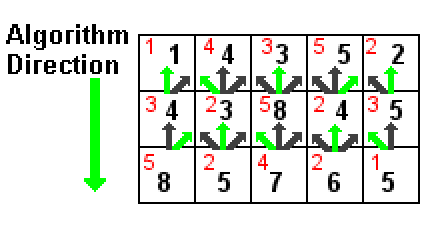
\includegraphics[scale=0.5]{dp1.png}
	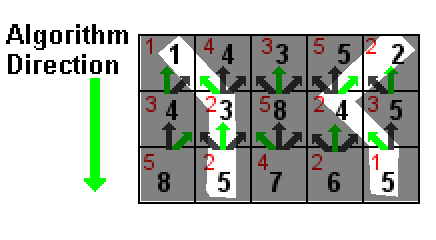
\includegraphics[scale=0.5]{dp2.png}
	\caption{Прямой и обратный ходы поиски шва}
\end{figure}

При сжатии изображения шов с минимальной энергией удаляется и размер изображения уменьшается на 1 по тому или иному направлению. Для возможности растягивать изображения была добавлена возможность работы с масками -- трехканальными RGB изображениями, где цвет каждого пиксела либо (255, 0, 0) (красный), либо (0, 255, 0) (красный), либо (0, 0, 0) (черный). Красные пиксели соответствуют части изображения, подлежащей обязательному удалению, зеленые -- обязательному сохранению. Для этого мы энергию соответствующих пикселей уменьшаем или увеличиваем на гарантированно большую величину -- $size\cdot 256$, где $size$ -- размер изображения. Тогда данные пиксели точно либо войдут в минимальные швы, вычисляемые при нескольких повторениях алгоритма, либо гарантированно останутся нетронутыми.

Работа с масками нам нужна при растяжении изображения, поскольку в этом случае мы вставляем между швом с минимальной энергией и его соседними пикселями справа или снизу шов с их усредненными значениями. Но в это случае минимальный шов всегда будет оставаться на месте и изображение будет расти неравномерно. Поэтому при помощи маски мы увеличиваем значение энергии точек данного шва.

Данное задание было выполнено. Наибольшие трудности вызвала отладка формирования поиска шва, поскольку, в отличие от предыдущего задания, требовались абсолютно точные координаты минимального шва, без какой-либо погрешности. Большое количество времени было потрачено на то, чтобы разобраться в готовом тестирующем коде как консольного, так и графического инструментов, в особенности работа с модулями PyQt4 и pickle. Потребовалось несколько раз менять приципы работы функций, вычисляющих энергию изображений и шов с минимальной энергией, несмотря на то, что теоретическая концепция не вызывает трудностей понимания.



\newpage
\subsection*{Практическое задание <<Распознавание автодорожных знаков>>}
\addcontentsline{toc}{subsection}{\protect\numberline{}Практическое задание <<Совмещение каналов изображения>>}%

В данном задании предлагалось реализовать классификацию автодорожных знаков с помощью SVM и
признаков HOG, а именно В данном задании необходимо написать собственную реализацию подсчёта гистограмм ориентированных
градиентов, и затем найти оптимальные параметры классификатора SVM.

Основной идеей алгоритма является допущение, что внешний вид и форма объекта на участке изображения могут быть описаны распределением градиентов интенсивности или направлением краев. Реализация этих дескрипторов может быть произведена путём разделения изображения на маленькие связные области, именуемые ячейками, и расчетом для каждой ячейки гистограммы направлений градиентов или направлений краев для пикселей, находящихся внутри ячейки. Комбинация этих гистограмм и является дескриптором. Для увеличения точности локальные гистограммы подвергаются нормализации по контрасту.

Реализация извлечения признаков HOG вызвало большие трудности из-за своей теоретической сложности и отсутствия понимания о практической реализации. Вследствии этого было рассмотрено большое количество сторонних источников -- статей, исходных кодов библиотеки $skimage$ и различных имплементаций алгоритма, доступных на портале GitHub. Далеко не все сторонние источники имели информацию, оказавшуюся по-настоящему полезной, но некоторые помогли в реализации алгоритма, но реализации, которая за меня решала поставленную задачу (классификации знаков) найдено не было, поскольку авторы синонимичных проектов использовали программные компоненты, не предоставляемые тестовой системой (в частности специализированная библиотека для компьютерного зрения OpenCV). Наиболее важное значение посторонних источников заключалось в принятии решения об использовании определенных значений для параметров алгоритма, поскольку не раз утверждалось о получении таких значений эмпирическим путем в прошлом и их широком использовании в настоящем.

Был реализован алгоритм подсчета гистограмм ориентированных градиентов:
\begin{enumerate}
	\item На входе имеем квадратное изображение дорожного знака. Изменим его разрешение до $64\times64$ пикселя. Так как мы будем работать с полутоновой интерпретацией изображения, игнорируя цветность, такой размер наиболее оптимален для распознавания признаков.
	 \item Подсчет значения градиентов. Для этого вычисляются производные изображения $I_x$ и $I_y$ путем свертки c обычными разностными ядрами:
	 \[
	 D_x=(-1, 0, 1), \ D_y=(-1, 0, 1)^T
	 \]
	 Затем вычисляются модуль и направление градиента в каждой точке, после чего угол направления зеркалируется, помещаясь в диапозон от 0 до $\pi$:
	 \[
	 |G|=\sqrt{I_x^2+I_y^2}, \ \Theta=\arctan2\left(\frac{I_y}{I_x}\right)
	 \]
	 \item Разбиваем изображение на ячейки размера $8\times8$ пикселей, и для каждой из них считаем гистограмму градиентов -- вектор длины 9, состоящий из <<корзин>>, каждая из которых соответствует углам $0, 20, 40, 60 \dots 160$ (в градусах). То есть для каждого пикселя мы переводим его направление в градусы и пропорционально распределяем значение модуля градиента по корзинам, отвечающим за соседние углы (числа в корзинах суммируются) (см. рис 4).
	 
	 \begin{figure}
	 	\centering
	 	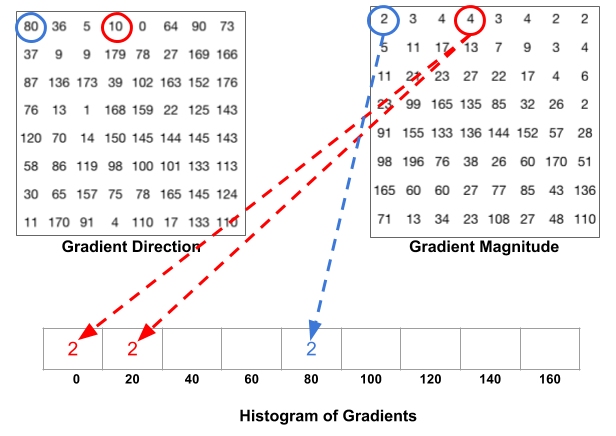
\includegraphics[scale = 0.5]{hog-histogram-1.png}
	 	\caption{Вычисление гистограммы для ячейки}
	 \end{figure}
 
	 \item Ячейки объединяются в блоки размером $16\times 16$, блоки могут пересекаться.
	 Гистограммы различных ячеек в блоке конкатенируются в вектор и нормируютсяб затем векторы каждого блока конкатенируются в один большой вектор, который и будет дескриптором изображения;
\end{enumerate}

	После этого встала задача подборки параметров классификатора SVM. В качестве базы была взята линейная модель. После некоторого подбора параметров была выбрана такая конфигурация, что точность классификатора была равна 99.7\% на публичной тестовой выборке, но 91.2\% на скрытой, что не является достаточно хорошим результатом. Возможным улучшением такого результата могла бы  быть более масштабная экспериментальная деятельность, например, разработка ядра для нелинейной модели, либо же использование иных структур, используемых в машинном обучении. Однако возможной причиной я считаю недостаточное экспериментирование с кросс-валидацией линейной модели, поскольку значительное время я потратил на алгоритм HOG.


\newpage
\section*{Заключение.}
\addcontentsline{toc}{section}{\protect\numberline{}Заключение.}%
В ходе учебной практики были выполнены практически все поставленные задачи:
\begin{enumerate}
	\item Произошло ознакомление с теоретическими основами компьютерного зрения и машинного обучения, историей становления данных областей знаний, основными понятиями и методами применимыми в них;
	\item Практическое задание <<Совмещение каналов изображения>> полностью выполнено и решение прошло все тесты;
	\item Практическое задание <<Контекстно-зависимое масштабирование изображений>> полностью выполнено и решение прошло все тесты;
	\item Практическое задание <<Распознавание автодорожных знаков>> не выполнено на полный балл (точность на скрытой тестовой выборке -- 91,2\%  против 93\% запрашиваемых). Есть понимание причин недостатков решения.
\end{enumerate} 

 Был получен опыт разработки приложений на языке Python, решения задач из области обработки изображений и их классификации, поиска и изучения научных статей, технической документации.

Полученные знания станут полезной базой для дальнейшего углубленного изучения области компьютерного зрения. На основании происхождения этой области и характере задач, которые в ней ставятся, можно сделать вывод, что методы, используемые для решения задач, в основном все еще существуют в экспериментальном виде, и дальнейшее изучение предполагает ознакомление с каждым из этих методов, поскольку на данный момент не практически не существует универсальных приемов, обобщающих задачи разных классов.

А полученный опыт прохождения практики позволяет сделать вывод о необходимости более творческого, экспериментального подхода к решению задач из области искусственного интеллекта и компьтерного зрения, в частности.

\newpage

%\nocite{*}
\section*{Список использованных источников и материалов.}
\addcontentsline{toc}{section}{\protect\numberline{}Список использованных источников и материалов.}
\begin{enumerate}
	\item Курс видеолекций А.С. Конушина <<Введение в компьютерное зрение и глубинное обучение>> --- \url{https://www.youtube.com/playlist?list=PLbwKcm5vdiSYL_yEwQ6JIICBA4dMtHNxo}
	\item Слайды к видеолекциям -- \url{cv-gml.ru}
	\item Документация библиотеки NumPy -- \url{https://docs.scipy.org/doc/numpy/reference/}
	\item Документация библиотеки scikit-image -- \url{http://scikit-image.org/}
	\item Документация библиотеки scikit-learn -- \url{http://scikit-learn.org/stable/index.html}
	\item Shai Avidan, Ariel Shamir -- <<Seam Carving for Content-Aware Image Resizing>> --- \url{http://www.faculty.idc.ac.il/arik/SCWeb/imret/imret.pdf}
	\item <<Histogram of Oriented Gradients>>, December 6, 2016 By Satya Mallick --- \url{http://www.learnopencv.com/histogram-of-oriented-gradients/}
\end{enumerate}
\end{document}
